\documentclass[../../../../main.tex]{subfiles}
\begin{document}

\begin{flushright}
\footnotesize\textit{【自動文字起こし・要確認】}
\end{flushright}

[解] 題意の円を $C$ とおく．
\begin{align*} C \equiv (x-2)^2+(y+1)^2=4 \end{align*}
から, $O(2, -1), \, r=2$ である．そこで,
\begin{align*} \vec{OP} = \begin{pmatrix} x-2 \\ y+1 \end{pmatrix} \end{align*}
だから, $\vec{OQ} = k\vec{OP} \quad (k>0)$ とおけることより,
\begin{align*} |\vec{OP}| \cdot |\vec{OQ}| = k \{ (x-2)^2+(y+1)^2 \} = 4 \quad (\because \text{題意}) \end{align*}
$O \ne P$ から
\begin{align*} k = \frac{4}{(x-2)^2+(y+1)^2} \end{align*}
だから,
\begin{align*} \vec{OQ} = \begin{pmatrix} X-2 \\ Y+1 \end{pmatrix} = \frac{4}{(x-2)^2+(y+1)^2} \begin{pmatrix} x-2 \\ y+1 \end{pmatrix} \end{align*}
である．成分を比較して
\begin{align*}
\begin{cases}
X = \dfrac{4(x-2)}{(x-2)^2+(y+1)^2} + 2 \\[10pt]
Y = \dfrac{4(y+1)}{(x-2)^2+(y+1)^2} - 1
\end{cases}
\quad \text{(1)}
\end{align*}

(2) $x \in \mathbb{R}, \, y=0$ だから, (1) より
\begin{align*}
\begin{cases}
X-2 = \dfrac{4(x-2)}{(x-2)^2+1} \\[10pt]
Y+1 = \dfrac{4}{(x-2)^2+1}
\end{cases}
\quad \dots (*)
\end{align*}
$Y \ne -1$ だから (第2式より), 第2式を変形して,
\begin{align*} (x-2)^2+1 = \frac{4}{Y+1} \end{align*}
第1式に代入して,
\begin{align*} X-2 = (Y+1)(x-2) \end{align*}
\begin{align*} \therefore x-2 = \frac{X-2}{Y+1} \quad (\because Y \ne -1) \end{align*}
だから, $(*)$ に代入して
\begin{align*} Y+1 = \frac{4}{\left( \dfrac{X-2}{Y+1} \right)^2 + 1} \end{align*}
\begin{align*} \therefore (X-2)^2 + (Y+1)^2 = 4(Y+1) \quad (\because Y \ne -1) \end{align*}
\begin{align*} (X-2)^2 + (Y-1)^2 = 4 \quad \dots \text{①} \end{align*}
又, $(*)$ 及び $x \in \mathbb{R}$ から,
\begin{align*} 0 < Y+1 \le 4 \quad \therefore -1 < Y \le 3 \end{align*}
に注意して, $(X, Y) \ne (2, -1)$ である．以上から
\begin{align*} (X-2)^2 + (Y-1)^2 = 4 \quad ((X, Y)=(2, -1) \text{を除く})  \end{align*}

\begin{figure}[htb]
\begin{center}
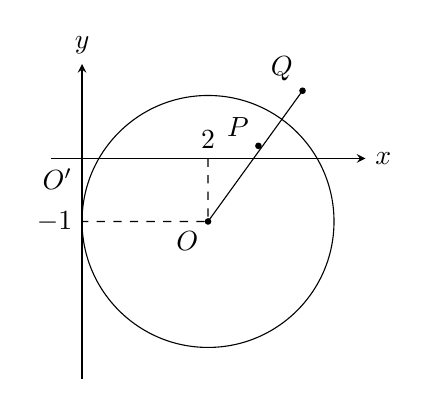
\begin{tikzpicture}[scale=0.8, >=stealth]
  \draw[->] (-0.5,0) -- (4.5,0) node[right] {$x$};
  \draw[->] (0,-3.5) -- (0,1.5) node[above] {$y$};
  \node[below left] at (0,0) {$O'$};
  \coordinate (O) at (2,-1);
  \draw[dashed] (2,0) node[above] {$2$} -- (O) -- (0,-1) node[left] {$-1$};
  \draw (O) circle (2);
  \fill (O) circle (1.5pt) node[below left] {$O$};
  \coordinate (P) at (2.8,0.2);
  \coordinate (Q) at (3.5,1.075);
  \draw (O) -- (Q);
  \fill (P) circle (1.5pt) node[above left] {$P$};
  \fill (Q) circle (1.5pt) node[above left] {$Q$};
\end{tikzpicture}
\end{center}
\caption{点$(X,Y)$の軌跡（円）の図示}
\end{figure}

\end{document}
